\apendice{Documentación técnica de programación}
Este apartado sirve para especificar y resumir la documentación técnica referente a la parte de desarrollo del código fuente de la aplicación, la instalación de Green In House realizada de cero y la ejecución de pruebas de sistema.
\section{Introducción}
En los siguientes apartados queda recogida la documentación respecto a las librerías que se utilizan en Green In House, las tecnologías que se utilizan y un manual de como habría que realizar de cero la instalación para poder replicar Green In Hosue. también está incluido un resumen de las pruebas de sistema que se han realizado.
\section{Estructura de directorios}
Este apartado ha sido descrito anteriormente en el apartado \textbf{C\_Diseño} en la sección \textbf{Diseño arquitectónico} en la subsección \textbf{Patrón de diseño MVC (Modelo-Vista-Controlador)}. Se ha decidido redactar en dicho apartado, ya que la estructura de directorios ha sido diseñada haciendo uso de las recomendaciones de segmentación de funciones que propone dicha metodología.

La estructura de los módulos que conforman Green In House está recogida en el siguiente diagrama de paquetes.

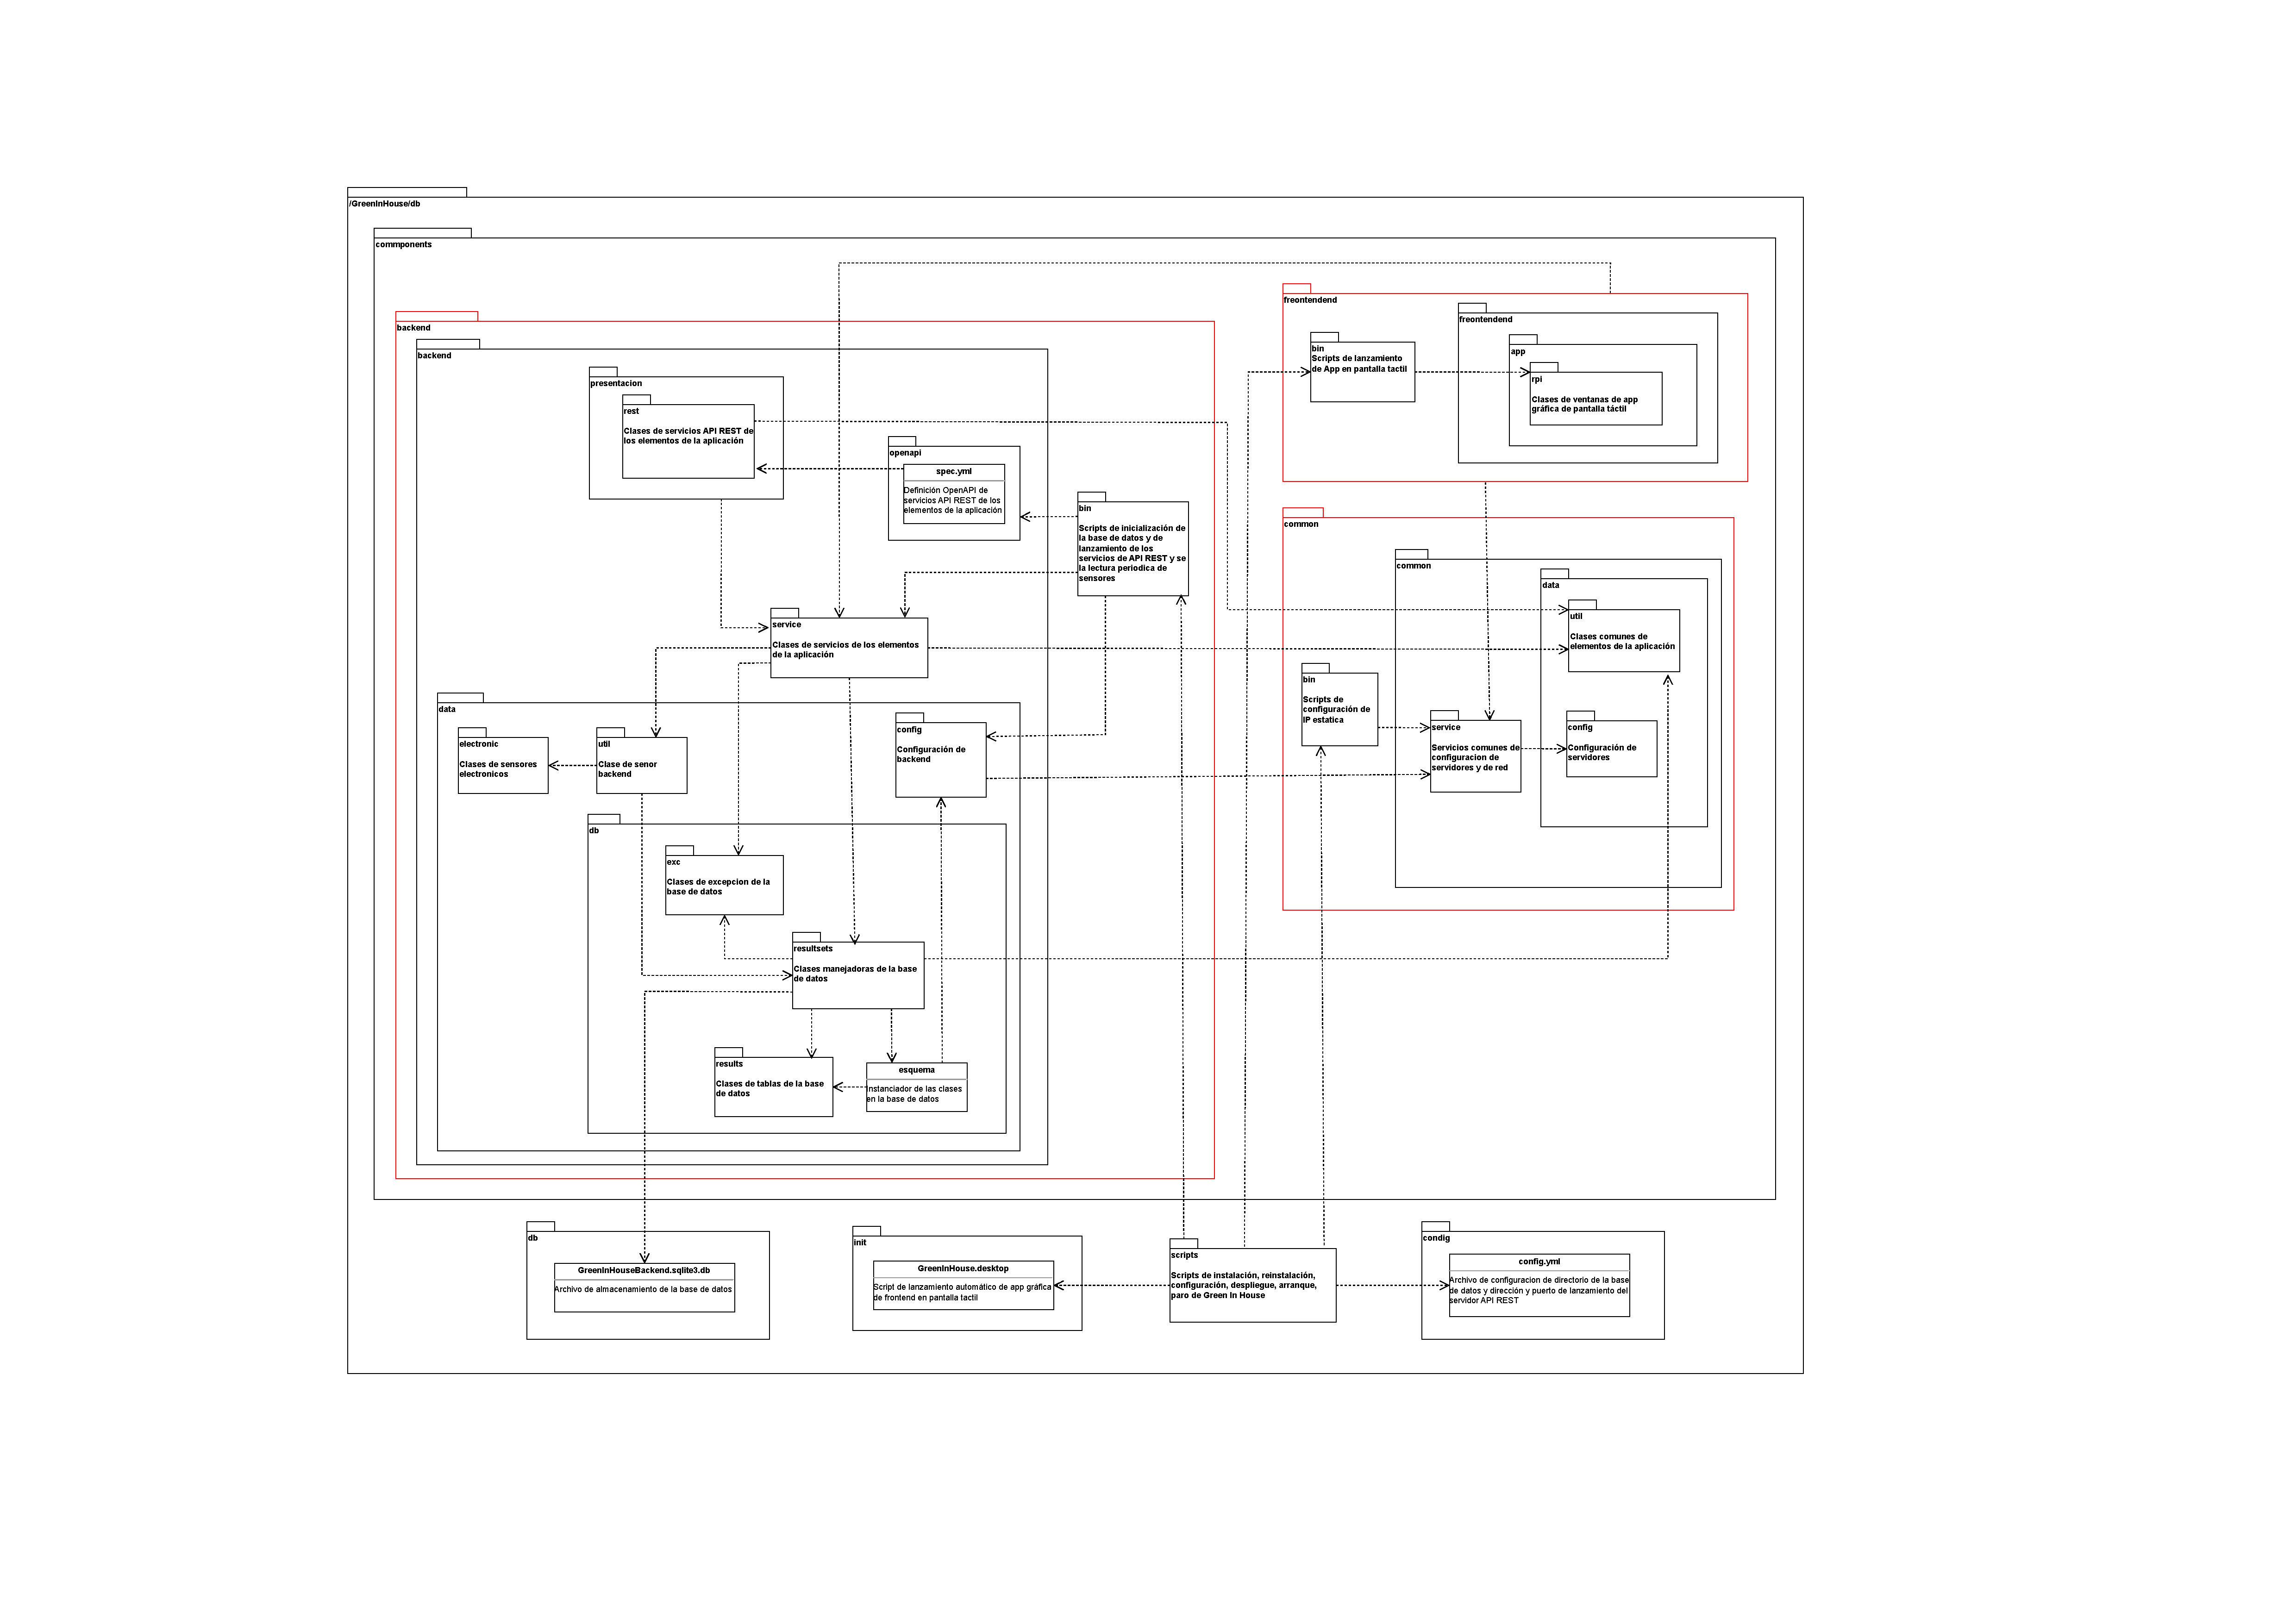
\includepdf[pages=1,fitpaper]{diagrama_de_paquetes_pdf}   
    
\section{Manual del programador}
Para desarrollar el código de Green In House se han utilizando las libreías SQLAlchemy, Adafruit Circuit Python, OpenAPI, y Thinter las cuales de talla a continuación como han sido utilizadas.

    \subsection{SQLAlchemy: Librería de base de datos en Python}
    Green In House utiliza SQLAlchemy \cite{wiki:sqlalchemy} para interactuar con una base de datos SQLite3. En esta base de datos están alojadas las tablas con las que trabaja Green In House, las cuales son:
    \begin{itemize}
        \item Sensores
        \item Registros Sensores
        \item Plantas
        \item Tipos Plantas
        \item Sensores Plantas
        \item Consejos Plantas
        \item Consejos Tipo Plantas
    \end{itemize}
    Cada una de estas tablas tiene implementada una clase intermediaria propia que se encarga de gestionar las transacciones con la base de datos y de construir el objeto python con los datos de las filas de su tabla correspondiente, y de almacenar los datos en las tablas correspondientes de los objetos python creados por la aplicación. 
    Para poder manejar los datos de la base de datos de manera cómoda, Green In House tiene una serie de servicios implementados que se encarga de gestionar las conexiones con la base de datos, delegando las transacciones en las clases manejadoras anteriormente mencionadas.

    \subsection{Adafruit - CircuitPython: Librería de sensores y actuadores en Python}
    Green In House utiliza la librería CircuitPyhon de Adafruit \cite{wiki:adafruit_circuit_python} para interactuar con los sensores electrónicos del sistema y leer de manera cómoda y sencillas sus valores. Green In House está preparada para comunicarse con los siguientes tipos de sensores:
       \subsubsection{MCP3008: Conversor de 8 señales analógicas a digital (ADC)}
        El MCP3008 \cite{wiki:mcp3008} es un conversor analógico-digital (ADC) de 10 bits y 8 canales. Esto significa que puede tomar hasta 8 señales analógicas diferentes y convertirlas en valores digitales.
        La resolución de 10 bits del MCP3008 indica que puede representar la señal analógica en valores digitales de 0 a 1023. Esto proporciona una precisión suficiente para muchas aplicaciones, incluyendo la lectura de la mayoría de los sensores analógicos.
        Uno de los aspectos más atractivos del MCP3008 es que se comunica con la Raspberry Pi (o cualquier otro microcontrolador) a través del protocolo de interfaz periférica serial (SPI). Esto hace que sea relativamente sencillo de conectar y programar, y más sencillo aun si se utiliza una librería que implementa ya la comunicación con dicho módulo como hace CircuitPython de Adafruit. \cite{doc:mcp3008}
        %TODO explicar patillaje y meter foto
        \subsubsection{DHT11: Sensor de humedad y temperatura ambiente}
        El DHT11 \cite{wiki:dht11} es un sensor de temperatura y humedad que permite realizar lecturas de dichos parámetros mediante un microcontrolador, como Raspberry Pi. Este módulo es de bajo costo y de fácil uso, por lo es  una opción muy popular para proyectos de monitoreo ambiental. Además la librería CircuitPython de Adafruit \cite{doc:mcp3008} cuenta con módulos ya programados para trabajar de manera muy sencilla con este sensor.
        El DHT11 es capaz de medir temperaturas entre 0 y 50 grados Celsius con una precisión de ±2 grados, y humedad relativa entre 20 y 80\% con una precisión de ±5\%.
        El módulo DHT11 utiliza un sensor capacitivo para la medición de la humedad y un termistor para la medición de la temperatura. Este sensor entrega una señal digital que puede ser leída directamente por la Raspberry Pi sin necesidad de convertirla mediantes un ADC.
        %TODO explicar patillaje y meter foto
        \subsubsection{FC28: Sensor de humedad de tierra de la maceta}
        El módulo FC28 es un sensor de humedad del suelo muy utilizado en proyectos relacionados con la jardinería automatizada y el monitoreo del suelo. Este dispositivo tiene la capacidad de medir la cantidad de agua presente en el suelo, permitiendo tener un conocimiento preciso de las condiciones de humedad de la tierra en la que está sembrada la planta. Este sensor entrega una señal analógica, por lo que se necesita convertirla mediante ADC a una señal digital para que pueda ser leida por la Raspberry Pi.
        %TODO explicar patillaje y meter foto
        \subsubsection{LDR: Sensor de luminosidad ambiente}
        Un LDR, o fotoresistor es un dispositivo que varía su resistencia en función de la cantidad de luz que incide sobre él. Sin embargo, es importante tener en cuenta que un LDR no mide directamente los lúmenes, la cual es una unidad de flujo luminoso. Un LDR mide la intensidad de luz de una manera no lineal y no opera en una frecuencia en particular. 
        Para obtener una estimación de la luz en términos de lúmenes, se ha seguido el siguiente proceso:    
        \begin{enumerate}    
            \item \textbf{Configuración del circuito:} 
            Conexión de un LDR y una resistencia fija en un circuito divisor de voltaje. Ambos extremos del LDR y la resistencia se conectan a una fuente de alimentación (en este caso a los 5V de la Raspberry Pi), y el otro extremo del LDR se conecta al otro extremo de la resistencia y a tierra (GND). De esta forma, el voltaje entre el LDR y la resistencia se puede medir y estará relacionado con la resistencia del LDR.   
            \item \textbf{Medición del voltaje:} 
            Este voltaje se mide con un ADC (Convertidor Analógico a Digital) en la Raspberry Pi. El modelo de Raspberry Pi utilizado o dispone de un ADC incorporado, por lo que se utiliza el ADC externo MCP3008, explicado anteriormente.        
            \item \textbf{Conversión del voltaje a resistencia:} 
            Conociendo el voltaje de la fuente de alimentación (V), el voltaje medido (Vout) y la resistencia seleccionada (R), se calcula la resistencia del LDR (Rldr) utilizando la fórmula: Rldr = R * ((V / Vout) - 1).        
            \item \textbf{Calibración del sensor:} 
            Para convertir la resistencia del LDR a lúmenes, hay que calibrar el sensor. Para ello, es necesario utilizar una fuente de luz con una salida conocida en lúmenes y medir la resistencia del LDR a diferentes niveles de luz. De esta forma, se puede crear una tabla de correspondencia entre la resistencia del LDR y los lúmenes.   
            \item \textbf{Conversión de resistencia a lúmenes:} 
            Con la tabla de correspondencia, se puede convertir las medidas de resistencia del LDR a lúmenes, aunque la fiabilidad de la medida depende mucho de lo bien que se haya realizado el proceso de calibración.
        \end{enumerate}        
        Es importante tener en cuenta que este método proporciona una medida aproximada y tiene sus limitaciones. Los LDR son sensibles a diferentes longitudes de onda de luz de diferentes maneras, por lo que diferentes tipos de luz (como la luz del sol, la luz fluorescente, etc.) darán diferentes lecturas.   
        %TODO explicar patillaje y meter foto
        \subsubsection{BH1750: Sensor de luminosidad ambiente.}  
        El módulo BH1750 es un sensor de luz ambiental de alta precisión muy utilizado en aplicaciones donde se requiere medir la intensidad de luz del entorno. Sirve para convertir la intensidad de luz que recibe en una señal digital que puede ser leída por un microcontrolador como Raspberry Pi.
        Este módulo tiene una alta precisión y resolución, pudiendo medir la intensidad de la luz en un rango desde 1 a 65535 lux. 
        Cuenta interfaz de comunicación I2C, que permite una integración sencilla con la Raspberry Pi y la posibilidad de conectar varios sensores en serie al mismo bus I2C, lo cual reduce la cantidad de pines utilizados en el microcontrolador. Este módulo puede tener 2 direcciones I2C distintas, dependiendo de si su patilla Dir se conecta a Vcc o a GND, por lo que esto permite tener 2 de estos módulos conectados en el mismo bus I2c.
        %TODO explicar patillaje y meter foto

    \subsection{OpenAPI: Librería de API REST en Python}
    Green In House utiliza el Microframework Connexion, el cual mapea el API REST especificado en el archivo spec.yml (mirar el apartado \textit{estructura de diretorios} para conocer su localización) con OpenAPI \cite{wiki:openapi} en Python, facilitando la creación de los \textit{endpoints} para que otras aplicaciones puedan conectar con el servicio, el cual es lanzado en el puerto 5000. Para poder hacer uso de estos \textit{endpoints} hay que hacerlo utilizando de base una de las siguientes urls: 
    \begin{itemize}
        \item http://192.168.1.240:5000/api/v1/
        \item http://greeninhouse:5000/api/v1/
    \end{itemize}
    Para poder ver wl Swager, la estructura de los \textit{endpoints} y ejemplos de uso, hay que hacerlo utilizando de base una de las siguientes urls: 
    \begin{itemize}
        \item http://192.168.1.240:5000/api/v1/ui/
        \item http://greeninhouse:5000/api/v1/ui/
    \end{itemize}
    \imagen{api_rest_gih}{Captura de pantalla del Swagger de la API REST de Green In House desarrollada con OpenAPI}{1}

    \subsection{TKinter:  Librería de interfaces gráficas en Python}
    Green In House utiliza la librería TKinter \cite{wiki:tkinter} para definir una aplicación gráfica multiventana que permite introducir en el sistema el nombre de la red WiFi del usuario y la contraseña de dicha red WiFi, así como reiniciar y apagar la maceta.
    \imagen{app_tkinter}{Captura de pantalla de la app gráfica de Green In House desarrollada en TKinter}{1}

\section{Compilación, instalación y ejecución del proyecto}
Para facilitar la instalación de Green In House en nuevos sistemas, cuenta con una gran variedad de scripts ya programados en Bash para realizar de manera automatizada la instalación de librerías, la generación y configuración de entornos virtuales, la instalación de dependencias en sus correctas versiones, la creación de la base de datos, la configuración de dirección IP estática del WiFi, el despliegue del código del programa en los entornos virtuales y la configuración de autoarranque del sevidor API REST, la lectura cíclica de sensores y el lanzamiento de la app gráfica en la pantalla táctil.
El directorio de despliegue en el que se almacenará toda la aplicación de Green In House tras su instalación por medio de los scripts facilitados se encuentra en la raíz del sistema y concretamente es \textbf{\texttt{/GreenInHouse}}. La estructura de directorios dentro de este directorio cambia ligeramente respecto a la del código fuente, pero se mantiene la misma estructura de paquetes para el funcionamiento de la aplicación. Se recomienda no modificar directamente los archivos del directorio \textbf{\texttt{/GreenInHouse}}, ya que al realizar un nuevo despliegue o instalación, las modificaciones en este directorio serán eliminadas. Si se quiere modificar el funcionamiento de la aplicación, habría que realizar dichas modificaciones en el código fuente descargado y posteriormente ejecutar el script de despliegue o instalación correspondiente.

    \subsection{Instalación del sistema operativo Raspbian}
    La instalación de Raspbian en la Raspberry Pi es un proceso muy sencillo. Solamente hay que seguir los siguiente pasos:    
        \begin{itemize}
            \item Descargar de la página web oficial de Raspberry el software Raspberry Pi Manager
            https://www.raspberrypi.com/software/
            \item Instalar el softeware Raspberry Pi Manager en un ordenador.
            \item Ejecutar el software Raspberry Pi Manager.
            \item Elegir la versión de sistema operativo que deseamos instalar. En mi caso he elegido Raspbian.
            \imagen{raspbian}{Captura de pantalla del instalador de Raspbian}{.6}
            \item Elegir el dispositivo de almacenamiento en el que instalarlo. En mi caso una tarjeta micro SD de 32 Gb.
            \item Una vez terminado el proceso de instalación, se introduce la tarjeta micro SD en la Raspberry, se le proporciona alimentación y la Raspberry comenzará a funcionar. 
        \end{itemize}
        \imagen{escritorio_raspbian}{Captura de pantalla del escritorio de Raspbian}{.6}

    \subsection{Necesidad de instalar un adaptador WiFi USB}  
    El modelo de Raspberry que utilicé para desarrollar Green In House es una Raspberry Pi 2b, el cual no cuenta con conexión WiFi, por lo que fue necesario utilizar un adaptador WiFi conectado por USB. Como adaptador WiFi USB utilicé el modelo 8812BU el cual dispone de conectividad a redes WiFi AC de alta velocidad. La instalación de este adaptador no está automatizada mediante un \textit{script} ya que no es estrictamente necesario realizar en todos los modelos de Raspberry Pi, además necesita reiniciar el sistema varias veces a lo largo de la instalación, por lo que no es posible ejecutarlo en un único \textit{script} de manera seguida. Debido a ello, su instalación manual queda reflejada a continuación. Es necesario contar con acceso a internet en la Raspberry para poder descargar el fichero, por lo que inicialmente será necesario conectarla por cable Ethernet:
    \begin{itemize}
        \item Ejecución del siguiente comando para realizar la actualización de las \textit{headers} del sistema y de lo módulos necesarios:
            \begin{itemize}
                \item \texttt{sudo apt install -y linux-headers raspberrypi-kernel-headers build-essential bc dkms git}
            \end{itemize}
        \item Reiniciar el sistema.
        \item Clonado del repositorio donde está almacenado su driver (para ello realicé un \textit{fork} de la versión de los drivers que funcionaron en mi sistema, ya que probé muchos hasta encontrar unos que funcionasen correctamente):
            \begin{itemize}
                \item \texttt{git clone https://github.com/ove1001/88x2bu-20210702}
            \end{itemize}
        \item Ejecutar el script de instalación alojado en el interior del repositorio descargado:
            \begin{itemize}
                \item \texttt{sudo ./install-driver.sh}
            \end{itemize}
        \item Reiniciar el sistema.
        \item Comprobar que el adaptador WiFi USB se reconoce correctamente:
            \begin{itemize}
                \item \texttt{lsub}
            \end{itemize}
        \item Editar el fichero de sistema que almacena las interfaces Ethernet: 
            \begin{itemize}
                \item \texttt{sudo nano /etc/network/interfaces}
            \end{itemize}
        \item Añadir en dicho fichero las siguientes lineas:
            \begin{itemize}
                \item \texttt{allow-hotplug wlan0}
                \item \texttt{iface wlan0 inet manual}
                \item \texttt{wpa-conf /etc/wpa\_supplicant/wpa\_supplicant.conf}
            \end{itemize}
        \item Reiniciar el sistema.
    \end{itemize}
    Tras este proceso el adaptador WiFi estará instalado y configurado para poder conectarse a una red WiFi mediante una dirección IP estática. Debido a algún tipo de bug en la interfaz gráfica, es posible que no se muestren las redes WiFi de alrededor, pero el adaptador WiFi funcionará correctamente. Para introducir las credenciales de la red WiFi se utilizará la App desarrollada en la pantalla táctil.

    \subsection{Instalación de Green In House en Raspberry Pi}
    Una vez instalado el sistema operativo Raspbian, lo que hay que hacer a continuación es encender la Raspberry Pi y descargar el código del proyecto del repositorio oficial de Green In House \cite{GreenInHouse:repo:Maceta}. 
    Una vez descargado el código fuente, dentro de la carpeta \texttt{scripts} se encuentran varios \textit{scripts} programados para realizar todas las tareas necesarias. 
    Entre los directorios del código fuente se encuentra la carpeta \texttt{config}, la cual contiene un archivo llamado \texttt{config.yml}. Este archivo contiene la información de la ruta donde se almacenará el archivo de la base de datos en el sistema y la dirección IP estática, máscara de red y puerta de enlace que se configurará en la Raspberry Pi durante la instalación. Se recomienda no cambiar los parámetros de este archivo, ya que inicialmente se definió con la idea de hacerlo modificable y que la aplicación se ejecutase acorde a lo establecido en dicho archivo, pero finalmente no ha sido posible por limitaciones técnicas. Estas limitaciones conciernen a la parte de la app móvil, ya que Android no es capaz de resolver las direcciones ip en base al \textit{hostname}. Debido a esto ha sido necesario establecer una IP estática en la Raspberry para el servidor API REST, y definir en el código Flutter de la app móvil, que el \textit{endpoint} base al que tiene que dirigir todas las \textit{API Calls} es 192.168.1.240, por lo que si se cambia la dirección IP de la Raspbery, la app móvil no será capaz de encontrar el servidor API REST y quedará inservible esta funcionalidad.

        \subsubsection{Scripts Bash de Green In House}
        Green In House cuenta con varios scripts Bash desarrollados para facilitar las tareas de instalación, despliegue, ejecución y parada de la aplicación. El nombre de todos los \textit{scripts} comienza por GIH- , haciendo referencia a que son tareas lanzadas para el funcionamiento de Green In House. Esto se ha determinado así para poder identificar fácilmente estas tareas en el programador de tareas de Raspbian y poder detener dichos procesos cuando sea necesario. Antes de lanzar una tarea, se realiza un intento de parada de la misma. Esto sirve para asegurar que no se lancen múltiples tareas para desarrollar el mismo trabajo, ya que eso ocasionaría inestabilidad en el sistema y pérdida de recursos.
        \begin{itemize}    
            \item Instalación de la aplicación (tanto la parte de \textit{backend} como de \textit{frontend}), generación de entornos virtuales de Python con la instalación de sus correspondientes dependencias, establecimiento de IP estática, configuración de los archivos de sistema pertinentes y configuración del arranque automático de los servicios de Green In House durante el arranque del sistema operativo. Estos scripts están escritos es Bash y es necesario ejecutarlos como superusuario, ya que necesitan generar y modificar archivos dentro de los directorios del sistema. Estos \textit{scripts} tardan bastante en ejecutarse y es necesario contar con conexión a internet. Es necesario reiniciar la Raspberry tras la instalación para que tengan efectos los cambios realizados en el sistema operativo. Todos ellos comprueban durante la instalación del sistema si existe el archivo de la base de datos \texttt{/GreenInHouse/db/GreenInHouseBackend.sqlite3.db} y si no está vacio. En caso contrario, se crea un nuevo achivo de base de datos y se ejecuta el \textit{script} python \texttt{GIH-backend-create-initial} almacenado en el directorio \texttt{backend/bin}, instanciando los tipos de plantas, la planta y los sensores establecidos por defecto en dicho script.
            \begin{itemize}
                \item \texttt{GIH-install.sh :} instalar todo el entorno de Green In House. 
                \item \texttt{GIH-install\_frontend.sh :} instalar el entorno de frontend de Green In House.
                \item \texttt{GIH-install\_backend.sh :} instalar el entorno de backend de Green In House.
                \item \texttt{GIH-reinstall.sh :} renistalar todo el entorno de Green In House.
                \item \texttt{GIH-reinstall\_cleand.sh :} renistalar todo el entorno de Green In House y borrar el archivo actual de la base de datos. 
                \color{red}(CUIDADO: el borrado es definitivo, no es posible recuperarla después). \color{black}
                \item \texttt{GIH-reinstall\_frontend.sh :} reinstalar el entorno de frontend de Green In House.
                \item \texttt{GIH-reinstall\_backend.sh :} reinstalar el entorno de backend de Green In House.
                \item \texttt{GIH-reinstall\_clean\_backend.sh :} renistalar el entorno de backend de Green In House y borrar el archivo actual de la base de datos. 
                \color{red}(CUIDADO: el borrado es definitivo, no es posible recuperarla después). \color{black}
            \end{itemize}
            \item Despliegue de cambios en el código de la aplicación. 
            \begin{itemize}
                \item \texttt{GIH-deploy\_all.sh :} desplegar todo el código fuente de Green In House a los entornos virtuales y actualizar sus dependencias.
                \item \texttt{GIH-deploy\_clean\_alll.sh :} desplegar todo el código fuente de Green In House a los entornos virtuales, actualizar sus dependencias y borrar la base de datos actual.
                \color{red}(CUIDADO: el borrado es definitivo, no es posible recuperarla después). \color{black}
                \item \texttt{GIH-deploy\_frontkend.sh :} desplegar todo el código fuente del \textit{frontend} al entorno virtual de \textit{frontend} y actualizar sus dependencias.
                \item \texttt{GIH-deploy\_backend.sh :} desplegar todo el código fuente del \textit{backend} al entorno virtual de \textit{backend} y actualizar sus dependencias.
                \item \texttt{GIH-deploy\_clean\_backend.sh :} desplegar todo el código fuente del \textit{backend} al entorno virtual de \textit{backend}, actualizar sus dependencias y borrar la base de datos actual.
                \color{red}(CUIDADO: el borrado es definitivo, no es posible recuperarla después). \color{black}
                \item \texttt{GIH-deploy\_spec\_yml\_backend.sh :} desplegar la especificación de la API REST al entorno virtual de \textit{backend} y actualizar sus dependencias.
            \end{itemize}  
            \item Configurar la dirección IP de la interfaz WiFi acorde a la que establece el archivo de configuración \texttt{config.yml} del directorio \texttt{/GreenInHouse/cfg/}
            \begin{itemize}
                \item \texttt{GIH-configure\_static\_ip.sh :} modificar la dirección IP estática de la interfaz WiFi. Ejecuta internamente el \textit{script} python \texttt{GIH-common-configure-static-ip} almacenado en el directorio \texttt{common/bin}.
            \end{itemize}
            \item Lectura de los sensores activos en el sistema y su correspondiente generación de lineas en la base de datos    
            \begin{itemize}
                \item \texttt{GIH-read\_sensors.sh :} leer los sensores activos del sistema y grabar sus registros en la base de datos. Ejecuta internamente el \textit{script} python \texttt{GIH-backend-read-sensors} almacenado en el directorio \texttt{backend/bin}.
            \end{itemize}
            \item Lectura de la base de datos para mostrarla por pantalla (principalmente tuilizado para pruebas)   
            \begin{itemize}
                \item \texttt{GIH-read\_db.sh :} mostrar por pantalla o por terminar el contenido de la base de datos de manera legible para las personas (frases redactadas en base a sus atributos). Ejecuta internamente el \textit{script} python \texttt{GIH-backend-read-db} almacenado en el directorio \texttt{backend/bin}.
            \end{itemize}
            \item Parada y arranque de los diferentes procesos en ejecución que controlan el funcionamiento de Green In House.    
            \item Arranque y parada de tareas para la ejecución de servicios de Green In House:
            \begin{itemize}
                \item \texttt{GIH-run\_api\_rest.sh :} arranca el servidor API REST en la dirección y puerto configurados (por defecto en \texttt{192.168.1.240:5000:/api/v1/} o \texttt{greeninhouse:5000:/api/v1/}). Ejecuta internamente el \textit{script} python \texttt{GIH-backend-api-rest} almacenado en el directorio \texttt{backend/bin}.
                \item \texttt{GIH-stop\_api\_rest.sh :} detiene el servidor API REST.
                \item \texttt{GIH-run\_read\_sensors\_periodically.sh :} arranca el servicio cíclico de lectura de sensores activos. Por defecto este servicio lee los sensores y almacena sus registros en la base de datos cada 10 minutos. Ejecuta internamente el \textit{script} python \texttt{GIH-backend-read-sensors} almacenado en el directorio \texttt{backend/bin}.
                \item \texttt{GIH-stop\_read\_sensors\_periodically.sh :} detiene el servicio cíclico de lectura de sensores activos.
                \item \texttt{GIH-run\_app\_rpi.sh :} arranca la aplicación gráfica de de la pantalla tactil. Ejecuta internamente el \textit{script} python \texttt{GIH-frontend-app-rpi} almacenado en el directorio \texttt{frontend/bin}.
                \item \texttt{GIH-stop\_app\_rpi.sh :} detiene la aplicación gráfica de de la pantalla tactil.
            \end{itemize}
            \item   
            \item Arranque de servicios de Green In House:
            \begin{itemize}
                \item \texttt{GIH-start\_all.sh :} arranca los servicios de frontend y backend.
                \item \texttt{GIH-stop\_all.sh :} detiene TODOS los servicios de Green In House (frontend, backend, instalación en curso y despliegue en curso).
                \item \texttt{GIH-stop\_except.sh :} detiene todos los servicios de Green In House (frontend, backend, instalación en curso y despliegue en curso) excepto los servicios que se pasen como argumentos de entrada al \textit{script}. Admite hasta tres argumentos de entrada. Un argumento de entrada puede ser una tarea en concreto (\texttt{GIH-read\_db.sh}) o un conjunto de tareas (\texttt{GIH-deploy} : todos los \textit{scripts} de despliegue).
                \item \texttt{GIH-stop\_process.sh :} detiene el servicio especificado. Admite hasta tres argumentos de entrada. Un argumento de entrada solo puede ser una tarea en concreto (\texttt{GIH-read\_db.sh}) o un conjunto de tareas (\texttt{GIH-deploy} : todos los \textit{scripts} de despliegue).
                \item \texttt{GIH-start\_frontend.sh :} arranca los servicios de frontend.
                \item \texttt{GIH-stop\_frontend.sh :} detiene los servicios de frontend.
                \item \texttt{GIH-start\_backend.sh :} arranca los servicios de backend.
                \item \texttt{GIH-stop\_backend.sh :} detiene los servicios de backend.
                \item \texttt{GIH-stop\_backend.sh :} detiene los servicios de backend.
            \end{itemize}    
            
        \end{itemize} 
        Estos \textit{scripts} están alojados en el directorio \texttt{scripts} del código fuente de Green In House. Tras la instalación de Green In House quedan alojado en el sirectorio \texttt{/GreenInHouse/script}
    
        \subsubsection{Configuración del sistema operativo Raspbian}
        La configuración de estos archivos se realiza automáticamente durante la ejecución de los \textit{scripts} de instalación y reinstalación. Para poder desplegar la aplicación de Green In House de manera automática al encender las Raspberry y poder configurar los parámetros del adaptadr WiFi, ha sido necesario modificar los siguiente ficheros de sistema: 
        \begin{itemize}
            \item \textbf{Cron y Crontab :} Estos archivos se encargan de la ejecución periódica de tareas por parte del sistema operativo. Se ha utilizado esta funcionalidad para desplegar el backend de la aplicación durante el arranque del sistema operativo, de tal manera que aunque no se inicie el entorno gráfico, los servicios de backend de Green In House se lanzarán igualmente.
            \item \textbf{\texttt{/etc/xdg/autostart :}} En este directorio se almacena el archivo de configuración \texttt{GreenInHouse.desktop}. Este archivo gestiona el arranque automático de la aplicación gráfica de la pantalla táctil de Green In House durante el arranque del entorno gráfico del sistema operativo. Este archivo de configuración es copiado a este directorio durante la instalación de Green In House desde el directo \texttt{init} del código fuente. Se recomienda no modificar este archivo para evitar corroemper el lanzamiento automático de la aplicación gráfica de Green In House.
            \item \textbf{\texttt{/etc/network/interfaces :}} en este archivo se almacena la configuración de las interfaces de red habilitadas en la Raspberry Pi. En mi caso, la interfaz WiFi está etiquetada como Wlan0.
            \item \textbf{\texttt{/etc/dhcpcd.conf :}} en este archivo se establece el funcionamiento del DHCP o la especificación de la IP estática definida para cada interfaz de red. En el caso de Green In House, se ha definido la IP stática 192.168.1.240/24 para la interfaz Wlan0.
            \item \textbf{\texttt{/etc/wpa\_supplicant/wpa\_supplicant.conf :}} en este archivo se almacenan las credenciales de las redes WiFi conocidas (los datos del SSID y la clave de la red WiFi que introduzca el usuario) con un formato determinado para que pueda ser utilizado por el sistema operativo.
        \end{itemize}
        La modificación de cualquiera de estos archivos requiere que se reinicie el sistema para que tengan efecto los cambios.

        \subsubsection{Utilización de Venv en Green In House}
        Green In House cuenta con 3 venvs \cite{wiki:venv} diferentes, de los cuales 2 están destinados al backend y 1 al frontend. 
        \begin{itemize}
            \item \textbf{venv de backend para lectura de sensores:} Este entorno virtual está destinado principalmente a gestionar el uso de la librería ADAFruit para leer los sensores electrónicos y la librería SQLAlchemy para almacenar los datos de los registros en la base de datos.
            \item \textbf{venv de backend para API REST:} Este entorno virtual está destinado principalmente a gestionar el uso de la librería OpenAPI, desplegando un servidor API REST, el cual gestiona las peticiones de datos externas e interactúa con la base de datos almacenando y recogiendo información mediante el uso de la librería SQLAlchemy.
            \item \textbf{venv de frontend para App gráfica de pantalla táctil:} Este entorno virtual está destinado principalmente a gestionar el uso de la librería TKinter, la cual se utiliza para desplegar una aplicación gráfica que permite al usuario interactuar con la Raspberry Pi e introducir los datos de la red WiFi de su hogar, para conectar el servidor Green In House a su red. También permite apagar y reiniciar el sistema.
        \end{itemize}

    \subsection{Configuración de SSH para desarrollo remoto en Raspberry Pi utilizando VSCode}
    A la hora de realizar el proyecto, la manera más cómoda de trabajar que he encontrado, ha sido desarrollar en remoto desde mi ordenador portátil utilizando una conexión SSH \cite{wiki:ssh} y el IDE de programación VSCode \cite{wiki:vscode}. Esto me ha permitido desplegar el directorio de trabajo de mi Raspberry Pi en el VSCode de mi ordenador, como si fuera parte de mi sistema local. Este apartado es solo para facilitar el desarrollo, no es necesario realizarle para ejecutar el programa de Green In House en la Raspberry Pi. 
    La configuración de este apartado requiere hacerse de manera interactiva, ya que hay que generar las claves privadas y públicas dentro de la Raspberry Pi, y esto requiere suminitar una clave de cifrado propia del desarrollador. Este sistema de conexión remota segura no puede automatizarse debido a esto, ya que si se queda \textit{hardcodeada} la clave de comunicación dentro del propio código de la aplicación, puede suponer un gran riesgo de seguridad. Por ello, este apartado es necesario realizarle a mano, aunque durante la instalación Green In House habilita todos los puertos de comunicación para asegurar poder comunicarse correctamente con todos los sensores (SSH, I2C, SPI, SERIAL, RGPIO). Para realizar la configuración de SSH y VSCode se ha seguido un tutorial de internet \cite{wiki:ssh_configuracion}, pero se deja reflejado en este apartado los pasos a seguir.
        \subsection{Configuración de SSH en Raspberry Pi}
        A continuación se detalla como se configuran las claves de acceso por SSH en la Raspberry Pi
        \begin{itemize}
            \item \textbf{Generar par de llaves SSH}
            \\ \texttt{ssh-keygen -t ed25519 -f ~/.ssh/GIH}
            \item Introducir nuestra frase clave utilizada para generar el par de claves privada-publica
            \item Volver a introducir la misma frase clave.
            \item \textbf{Añadir la llave privada a SSH Agent}
            \\ \texttt{ssh-add ~/.ssh/GIH}
            \item Introducir nuestra frase clave utilizada para generar el par de claves privada-publica
            \item \textbf{Copiar la llave pública a RPi}
            \item En el siguiente comando sustituir green-in-house por el nombre de usuario que se haya configurado en Raspbian para el usuario principal con el que arranca el sistema operativo por defecto.
            \\ \texttt{ssh-copy-id -i ~/.ssh/GIH.pub green-in-house@GreenInHouse}
            \item Introducir la clave del usuario especificado en el comando anterior
        \end{itemize}
        \subsection{Configuración de VSCode en ordenador}
        A continuación se detalla como se configura en VSCode el acceso por SSH a la Raspberry Pi.
        \begin{itemize}
            \item Abrir VSCode.
            \item Abrir una terminal de VSCode.
            \item \textbf{Instalar la extensión Remote - SSH}
            \item \texttt{code --install-extension ms-vscode-remote.remote-ssh}
            \item Cerrar y abrir VScode.
            \item \textbf{Configurar la conexión SSH}
            \item Pinchar en el icono de la tele con un circulo (señalado en la siguiente imagen) para acceder a las conexiones SSH y pulsar sobre el + (señalado en la siguiente imagen).
            \\ \imagen{SSH_VSCode1}{Captura de pantalla 1 de VSCode configurandon acceso por SSH.}{.4}
            \item En el cuadro que aparecerá escribir el usuario de la raspberry @ seguido del hostname o la dirección IP. En mi caso es:
            \\ green-in-house@GreenInHouse
            \\ \imagen{SSH_VSCode2}{Captura de pantalla 2 de VSCode configurandon acceso por SSH.}{.7}
            \item En el cuadro que aparecerá seleccionar el directorio en el que se almacenará la configuración SSH. Utilizar el directorio de nuestro usuario actual del ordenador. En mi caso es:
            \item \texttt{C:/Users/UX581/.ssh/config}
            \\ \imagen{SSH_VSCode3}{Captura de pantalla 3 de VSCode configurandon acceso por SSH.}{.7}
            \item Abajo a la derecha aparecerá un mensaje de que se ha agregado correctamente el host SSH.
            \\ \imagen{SSH_VSCode4}{Captura de pantalla 4 de VSCode configurandon acceso por SSH.}{.7}
            \item Si pulsamos en abrir configuración se mostrará un archivo con las siguientes lineas:
            \\ Host GreenInHouse
            \\ \hspace*{5mm}HostName GreenInHouse
            \\ \hspace*{5mm}User green-in-house
            \item Pinchar de nuevo en el icono de la tele con un circulo (señalado en la siguiente imagen) para acceder a las conexiones SSH y pulsar sobre la flecha ->(señalada en la siguiente imagen).
            \\ \imagen{SSH_VSCode5}{Captura de pantalla 5 de VSCode configurandon acceso por SSH.}{.4}
            \item En el cuadro que aparecerá introducir la contraseña del usuario de la raspberri en el que estamos intentador loguearnos:
            \\ \imagen{SSH_VSCode6}{Captura de pantalla 6 de VSCode configurandon acceso por SSH.}{.7}
            \item Abajo a la izquierda aparecerá un cuadrado azul que indica que estamos conectados por SSH al equipo remoto:
            \\ \imagen{SSH_VSCode7}{Captura de pantalla 7 de VSCode configurandon acceso por SSH.}{.7}
            \item Pulsando en archivo y en abrir carpeta nos permitirá abrir un directorio remoto y trabajar con él como de costumbre:
            \\ \imagen{SSH_VSCode8}{Captura de pantalla 8 de VSCode configurandon acceso por SSH.}{.5}
            \item En el cuadro que aparecerá introducir la ruta del directorio que queremos abrir. En mi caso es:
            \\ \texttt{/home/green-in-house/TFG/GreenInHouse\_PlantPot}
            \\ \imagen{SSH_VSCode9}{Captura de pantalla 9 de VSCode configurandon acceso por SSH.}{.7}
            \item Nos volverá a pedir introducir la contraseña del usuario de la Raspberry utilizado. Tras hacerlo se desplegará el directorio y sus archivos
            \\ \imagen{SSH_VSCode10}{Captura de pantalla 10 de VSCode configurandon acceso por SSH.}{.5}
            \item Una vez que accedamos a un directorio, al pulsar en el icono de la tele con el círculo para conectarnos a un servidor remoto, nos mostrará la dirección de los últimos direcctorios utilizados de dicho servidor remoto:
            \\ \imagen{SSH_VSCode11}{Captura de pantalla 11 de VSCode configurandon acceso por SSH.}{.5}
        \end{itemize}

    \subsection{Desarrollo de aplicación móvil en Flutter}
    Para desarrollar la aplicación móvil en Flutter \cite{wiki:flutter} se ha recurrido a la utilización de Flutter Flow \cite{wiki:flutter_flow}, el cual permite realizar el desarrollo de aplicaciones móviles basandose en el diseño de la interfaz. A medida que se va construyendo la interfaz gráfica, Flutter Flow va generando el código de la aplicación Flutter correspondiente. 
    Flutter Flow es una plataforma privada y cerrada, por lo que no permite compatir públicamente mi proyecto de Flutter Flow para que cualquier pueda continuar desarrollándole. Por suerte la versión especial que tengo concedida gracias a ser estudiante universitario, me concede acceso a sincronizar la app desarrollada en Flutter Flow con un repositorio GitHub. Gracias a eso todos los avances en la aplicación móvil son accesibles públicamente a través de su repositorio \cite{GreenInHouse:repo:AppMovil}. Esto tiene el impedimento de que únicamente de deja realizar \textit{push} de Flutter Flow al repositorio. En ningún caso Flutter Flow permite hacer \textit{pulls} de los cambios hechos desde otro IDE, por lo que obliga a desarrollar todo el proyecto dentro de su plataforma.
    Para poder continuar desarrollando este proyecto Flutter en un IDE como por ejemplo Android Studio, lo que hay que hacer sería hacer un fork del repositorio de GitHub de Green In House Mobile App, para poder tener una versión propia del código de la aplicación. Tras hacer el \textit{fork}, lo siguiente sería realizar un \textit{gitclone} desde Android estudio del repositorio creado. Esto se realiza desde la pestaña superior de git.
    \imagen{Android_Studio1}{Captura de pantalla 1 de Android Studio.}{.5}
    A continuación especificamos el repositorio que queremos clonar, la ruta local donde queremos clonarlo y generar el proyecto y damos al botón \textit{clone}.
    \imagen{Android_Studio2}{Captura de pantalla 2 de Android Studio.}{.5}
    Una vez hecho esto, nos aparecerá en el navegador de Android Studio la applicación Flutter. Estas aplicaciones se programan utilizando el lenguaje Dart \cite{wiki:dart}
        
\section{Pruebas del sistema}
No ha sido posible crear un sistema automatizado de prubeas para verificar la integridad del código, por lo que todas las pruebas de funcionamiento has sido realizadas a mano. Principalmente las pruebas que han sido ejecutadas son pruebas de integración, las cuales permiten validar el funcionamiento correcto de los módulos por separado, al comprobar que su funcionamiento en conjunto es correcto. 
Lo más óptimo habría sido diseñar un plan de pruebas automatizado de pruebas unitarias y otro de pruebas de integración, pero por motivos de falta de tiempo no ha sido posible realizar dichos planes de pruebas. Esto es una de las propuestas de líneas futuras.
Todas las pruebas se han realizado tanto utilizando los servicios del propio backend por terminal, como haciendo uso de los \textit{endpoints} de la API REST, ya que esto es lo realmente interesante, debido a que será la forma habitual de operar de los usuarios. 
%TODO